% \documentclass{report}
% 
% \usepackage{fancyhdr}
\usepackage{fourier-orns}
\usepackage{hyperref}%% To refrence links / jumps
\usepackage{chngcntr} %% For some extra counters numberings
\usepackage[a4paper, right = 0.5in, left = 0.5in,top = 1in , bottom = 1in]{geometry}
\usepackage{etoolbox} %% Provides like a language for advanced customization
\usepackage{datetime} %% For dates of course
\usepackage{lastpage} %% provides pages numbers
\usepackage[sc]{titlesec} %% modify titles
\usepackage{enumerate}
\usepackage{cancel}
\usepackage{tikzsymbols}
\usepackage[dvipsnames]{xcolor}
\usepackage{import}
\usepackage{pdfpages} %% include other pdfs
\usepackage{transparent} %% Transparency
\usepackage{xcolor}  %% Colors
\usepackage[many]{tcolorbox}
\usepackage[framemethod=TikZ]{mdframed}
\usepackage{amsmath,amsfonts,amsthm,amssymb,mathtools}
\usepackage{tikz}
\usepackage{bookmark}
\usepackage{graphicx}
\usepackage{mathpazo}

\usepackage{fontawesome5}

\linespread{1.5}


\titleformat{\chapter}[display]   
{\fontfamily{ppl}\selectfont\huge\color{YellowOrange!80!orange}} % Font style and size 
{\raggedleft\color{purple}\fontsize{70}{0pt}\selectfont\thechapter}   
{-1.5cm}    			                          % Space between the chapter number and title
{
	\begin{tikzpicture}[overlay]
		\node[anchor = west,yshift = 0.2cm,xshift = -1cm] {\fontsize{90}{20} $\int_{}^{} $};
		\node[yshift = 4cm, xshift = 17cm]   {\includegraphics[width = 4cm]{preview0}};
	\end{tikzpicture}
\hspace{1cm}\Huge\raggedright\MakeUppercase}

\titleformat{\section}[block]
{
\fontfamily{ppl}\selectfont\huge\color{YellowOrange!80!orange}
}
{
\color{purple}\fontsize{20}{0pt}\selectfont\thesection 
}
{0cm}
{
	\begin{tikzpicture}[overlay]
		\node[anchor = west,yshift = 0.2cm,xshift = -0.4cm, circle = 1pt] {};
	\end{tikzpicture}
}

\titlespacing*{\section}{0pt}{0.7cm}{1.5cm}


\newcommand{\divider}
{
	\begin{center}
	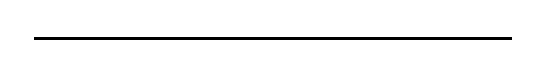
\begin{tikzpicture}
		\draw[thick, black] (0.25*\textwidth, 0) -- (0.75*\textwidth, 0);
		\node[rotate = 360 - 90, xshift = -0.6pt, yshift = 1pt] at (0.25*\textwidth,0){\decotwo};
		\node[rotate = 90, xshift = -0.6pt, yshift = 1pt] at (0.75*\textwidth,0){\decotwo};
	\end{tikzpicture}
	\end{center}
}

\pagestyle{fancy}

\newcommand{\lecday}[1][]
{
    \def\datee{#1}
    \fancyhead[L]{\datee}
}



\newcommand{\signature}
{
	\begin{tikzpicture}[remember picture,overlay]
		\node[fill = YellowOrange!20!white] at ([yshift = 1cm, xshift = -3cm]current page.south east) {\fontsize{10pt}{0pt}{\itshape Kara.$\mathcal{A}$}};
	\end{tikzpicture}
}

\AddToHook{shipout/background}{
  \begin{tikzpicture}[remember picture, overlay]
	  \node[] at ([yshift = 1.5cm,xshift = \textwidth /2 + 0.9cm]current page.south west) {\includegraphics[width = 0.5cm]{preview3}};
	  \node[] at ([yshift = 1.5cm,xshift = - \textwidth /2 - 0.9cm]current page.south east) {\includegraphics[width = 0.5cm]{preview4}};
  \end{tikzpicture}
}



\newtcolorbox[auto counter, number within = section]{remark}[1][]
{
       		title = Remark #1,
		enhanced,
		boxrule = 0pt,
		colback = white,
		breakable,
		arc = 4pt,
		colbacktitle = cyan,
		colback = cyan!5!white,
		segmentation style =
		{
			solid,cyan,thick,
		},
		attach boxed title to top left =
		{
			xshift = 0cm,
		},
		boxed title style =
		{
			boxrule = 0pt,
			sharp corners,
			drop fuzzy shadow = {cyan},
		},
		drop fuzzy shadow = {cyan!80!black},
}

\newtcolorbox[auto counter, number within = section]{theorem}[1][]
{                                      
		title = Theorem \thetcbcounter : #1,
		enhanced, 
		boxrule = 0pt,
		colback = white,
		breakable,
		arc = 4pt,
		colbacktitle = purple,
		colback = purple!5!white,
		segmentation style = 
		{
			solid, purple,thick,
		},
		attach boxed title to top left = 
		{
			xshift = 0cm, 
		},
		boxed title style = 
		{
			boxrule = 0pt,
			sharp corners,
			drop fuzzy shadow = {purple},
		},
		drop fuzzy shadow = {purple!80!black},
}

\newtcolorbox[auto counter, number within = section]{definition}[1][]
{                                      
		title = Definition \thetcbcounter : #1,
		enhanced, 
		boxrule = 0pt,
		colback = white,
		arc = 4pt,
		breakable,
		colbacktitle = YellowOrange!80!black,
		segmentation style = 
		{
			solid, YellowOrange,thick,
		},
		attach boxed title to top left = 
		{
			xshift = 0cm, 
		},
		colback = YellowOrange!5!white,
		boxed title style = 
		{
			boxrule = 0pt,
			sharp corners,
			drop fuzzy shadow = {YellowOrange!80!orange},
		},
		drop fuzzy shadow = {YellowOrange!80!black},
}

\newtcolorbox[auto counter, number within = section]{corollary}[1][]
{                                      
		title = corollary \thetcbcounter : #1,
		enhanced, 
		boxrule = 0pt,
		colback = white,
		arc = 4pt,
		breakable,
		colbacktitle = YellowOrange!80!black,
		segmentation style = 
		{
			solid, YellowOrange,thick,
		},
		attach boxed title to top left = 
		{
			xshift = 0cm, 
		},
		colback = YellowOrange!5!white,
		boxed title style = 
		{
			boxrule = 0pt,
			sharp corners,
			drop fuzzy shadow = {YellowOrange!80!orange},
		},
		drop fuzzy shadow = {YellowOrange!80!black},
}


\newtcolorbox{example}[1][]
{                                      
		title = Example,
		enhanced, 
		boxrule = 0pt,
		colback = white,
		arc = 4pt,
		segmentation style = 
		{
			solid, SpringGreen,thick,
		},
		breakable,
		colback = SpringGreen!5!white,
		colbacktitle = SpringGreen!80!black,
		attach boxed title to top left = 
		{
			xshift = 0cm, 
		},
		boxed title style = 
		{
			boxrule = 0pt,
			sharp corners,
			drop fuzzy shadow = {SpringGreen!80!orange},
		},
		drop fuzzy shadow = {SpringGreen!80!black},
}


\newcommand{\integral}[4]{\int\limits_{#1}^{#2} #4 d#3}
\newcommand{\limit}[3]{\lim\limits_{#1 \rightarrow #2} #3}
\newcommand{\strone}[2]{\left[ \begin{gathered}#1\\ #2\end{gathered} \right] }
\newcommand{\strtwo}[2]{\left\{ \begin{gathered}#1\\ #2\end{gathered} \right\} }
\newcommand{\strthree}[2]{\left\lfloor \begin{gathered}#1\\ #2\end{gathered} \right\rfloor }


\newcommand{\startbf}[1]{\text{\bfseries{#1}}}
\newcommand{\sett}[1]{\left\{ #1 \right\}}
\newcommand{\thesis}[1]{\left( #1 \right)}
\newcommand{\brkt}[1]{\left[ #1 \right]}
\newcommand{\floor}[1]{\left\lfloor #1 \right\rfloor}


\DeclareMathOperator{\img}{im} % Image
\DeclareMathOperator{\Img}{Im} % Image
\DeclareMathOperator{\coker}{coker} % Cokernel
\DeclareMathOperator{\Coker}{Coker} % Cokernel
\DeclareMathOperator{\Ker}{Ker} % Kernel
\DeclareMathOperator{\rank}{rank}
\DeclareMathOperator{\Spec}{Spec} % spectrum
\DeclareMathOperator{\Tr}{Tr} % trace
\DeclareMathOperator{\pr}{pr} % projection
\DeclareMathOperator{\ext}{ext} % extension
\DeclareMathOperator{\pred}{pred} % predecessor
\DeclareMathOperator{\dom}{dom} % domain
\DeclareMathOperator{\ran}{ran} % range
\DeclareMathOperator{\Hom}{Hom} % homomorphism
\DeclareMathOperator{\Mor}{Mor} % morphisms
\DeclareMathOperator{\End}{End} % endomorphism


\newcommand{\lm}{\ensuremath{\lambda}}
\newcommand{\eps}{\ensuremath{\epsilon}}
\newcommand{\veps}{\ensuremath{\varepsilon}}
\newcommand{\al}{\ensuremath{\alpha}}
\newcommand{\bb}{\ensuremath{\beta}}
\newcommand{\cc}{\ensuremath{\gamma}}
\newcommand{\dd}{\ensuremath{\delta}}
\newcommand{\DD}{\ensuremath{\Delta}}
\newcommand{\ff}{\ensuremath{\phi}}
\newcommand{\FF}{\ensuremath{\varphi}}

\newcommand{\RR}{\mathbb{R}}
\newcommand{\RO}{\mathcal{R}}
\newcommand{\EE}{\mathbb{E}}
\newcommand{\CC}{\mathbb{C}}
\newcommand{\RW}{\mathbb{R}^2}
\newcommand{\RT}{\mathbb{R}^3}
\newcommand{\RN}{\mathbb{R}^n}
\newcommand{\DS}{\mathcal{D}}

\newcommand{\KK}{\mathbb{K}}
\newcommand{\KW}{\mathbb{K}^2}
\newcommand{\KT}{\mathbb{K}^3}
\newcommand{\KN}{\mathbb{K}^n}

\newcommand{\NN}{\mathbb{N}}

\newcommand{\PS}{\mathcal{P}}
\newcommand{\AS}{\mathcal{E}}
\newcommand{\FS}{\mathcal{F}}
\newcommand{\LS}{\mathcal{L}}
\newcommand{\MS}{\mathcal{M}}


















\lecday[2025-05-08]

% \begin{document}

\begin{theorem}[(Hahn-Banach)]
	Let $E $ be a $\KK $-vector space $(\KK = \RR \text{ or } \CC )  $  
	and $H $ be a vector subspace of $E $ let 
	also 
	$ N : E \longrightarrow [0,\infty) $ 
	be a seminorm on $E $ and 
	$ f : H \longrightarrow \KK $ be a linear
	form on $H $, satisfying 
	\[
	\left| f(x)  \right| \leq N(x)  \quad \quad 
	(\forall  x \in  E) 
	\] 
	then there exist a $\KK $-linear form 
	$ \overset{\sim}{f}  : E \longrightarrow \KK $,
	extending $f $ and satisfying 
	\[
	\overset{\sim}{f} \leq N(x) \quad \quad (\forall  x \in  E)
	\]
\end{theorem}
\begin{proof}
\textbf{Case 01 :} \\
If $\KK = \RR $  
since we have for all $x \in  H $, 
\[
f(x) \leq \left| f(x)  \right| \leq N(x) 
\]
then by applying Theorem $1 $ for 
$p = N $, we find that there exist a linear form
$ \overset{\sim}{f}  :  E \longrightarrow  \RR $ 
extending $f $ and satisfying 
\[
\forall x \in  E : 
\overset{\sim}{f} (x)  \leq  N(x)  \quad \quad  (1) 
\]
By applying $(1)$ for $(-x)  $   instead of $x$, we get, 
\begin{align*}
	\overset{\sim}{f} (-x) &\leq  N(-x) = N(x)   \\
	- \overset{\sim}{f} (x)  &\leq 
	N(x) \\
	\overset{\sim}{f} (x)  & \geq 
- N(x)  \quad  \quad  (2) 
\end{align*}
from $(1)$ and $(2)$, we have 
\begin{align*}
	&\iff  - N(x)  \leq  \overset{\sim}{f} (x)   \\
	&\iff  \left| \overset{\sim}{f} (x)  \right| \leq 
	N(x) 
\end{align*}
\textbf{Case 02: } \\
Define 
\[
\begin{array}{cccc}
      g : &  H  & \longrightarrow & \RR  \\

           &  x  & \longmapsto     & g(x) := Re f(x) = \frac{f(x) + \overline{f(x) }}{2} \\ 
\end{array}
\]
Its clear that $g $ is an $\RR  $-linear form on $H $, next we have for all 
$x \in  H $, 
\begin{align*}
	\left| g(x)  \right| =
	\left| Re(f(x) )  \right| & \leq 
\left| f(x)  \right| \\
				  & \leq 
				  N(x) 
\end{align*}
for all $x \in  H $, 
\[
	\left| g(x)  \right| \leq 
	N(x) 
\]
so we can apply the result of the first case, 
for the linear form $g $ on $H $, we find that 
$ \exists \overset{\sim}{g}  : E \longrightarrow \RR  $ 
an $\RR$-linear extending $g $, and satisfying, 
\[
\forall  x \in  E: \quad 
\left| \overset{\sim}{g} (x)  \right| \leq 
N(x) 
\]
Furthermore, we have, for all $x \in H$, 
\begin{align*}
	g(ix)  &= 
	Re ( \overline{f}(ix) )  \\
	       &=
	       Re (i f(x) )  \\
	       &= - Im f(x)  \\
	       & \implies 
	       Im f(x)  = - g(ix) 
\end{align*}
Then for all $x \in  H $, 
\begin{align*}
	f(x)  &= 
	Re f(x)  + i Imf(x)  \\
	      &= g(x) - i g(ix) 
\end{align*}
Thus, we have for all $x \in  H $, 
\[
f(x) = g(x) - i g(ix)  \quad \quad  (1) 
\]
therefore define,
$ \overset{\sim}{f}  : E \longrightarrow \CC  $, by, 
\[
\overset{\sim}{f} (x)  = 
\overset{\sim}{g} (x)  - i \overset{\sim}{g} (ix) 
\]
\begin{center}
	\textbf{
	We will prove that it's an extension
	}
\end{center}
\begin{enumerate}[(1)]
\item Show that $\overset{\sim}{f}$ extends $f$. 
\item Show that $\overset{\sim}{f}  $ is $\CC$-linear.
\end{enumerate}
\begin{proof}
Since $\overset{\sim}{g}  $  is $\RR  $-linear then 
$\overset{\sim}{f}  $  is obviously $\RR$-linear. So, to show that 
$\overset{\sim}{f}  $  is $\CC$-linear it sufficies to show that 
\[
\overset{\sim}{f} (ix)  = i 
\overset{\sim}{f} (x)  \quad \quad  (\forall  x \in  E) 
\]
for all $x \in  E $, we have, 
\begin{align*}
	\overset{\sim}{f} (ix)  &= \overset{\sim}{g} (ix)  - 
	i \overset{\sim}{g} (-x)  \\
				&= 
		\overset{\sim}{g} (ix)  + i 
		\overset{\sim}{g} (x) \\
				&= i \left( 
					\overset{\sim}{g} (x)  -
					i \overset{\sim}{g} (ix) 
				\right) = i 
				\overset{\sim}{f} (x) 
\end{align*}
as required, then $ \overset{f}{\sim}  $ is $\CC  $-linear.
\end{proof}
Now we have to show that 
\[
\left| 
\overset{\sim}{f}  (x)  \leq N(x)  \quad \quad  (\forall  x \in  E) 
\right|
\]
Finally, for all $x \in  E $, by writting the complex number
 $\overset{\sim}{f}(x)$ in it exponential form, say, 
 \[
 \overset{\sim}{f} (x)  = 
 \left| \overset{\sim}{f} (x)  \right| e^{i \theta} \quad \quad 
 (\theta \in  \RR ) 
 \]
 we have, 
 \begin{align*}
 \left| 
 \overset{\sim}{f}(x)  
 \right| &= 
 \overset{\sim}{f} (x) e^{-i \theta} \\
	 &= 
	 \overset{\sim}{f} (x e^{-i \theta})  \\
	 &= 
	 Re \overset{\sim}{f} (x e^{-i \theta}) \\
	 &= 
	 \overset{\sim}{g} (x e^{-i \theta})  \\
	 & \leq 
	 N(xe^{-i \theta})  = \left| e^{-i \theta} \right| N(x)  = N(x) 
 \end{align*}
 Thus \[
 \left| \overset{\sim}{f} (x)  \right| \leq N(x) \quad \quad  (\forall  x \in  E) 
 \]
 as required, thus this completes the proof.
\end{proof}
\begin{theorem}[Hahn-Banach]
	Let $E $ be a N.V.S over a field $\KK = \RR  $ or $\CC  $ and 
	$H $ be a non zero subspace of $E $, then for all $f \in  H'=
	\mathcal{L} (H,K) $ there exists 
	\[
	\overset{\sim}{f} \in  E' = 
	\mathcal{L} (E, \KK) 
	\] 
	extending $f $ and satisfying, 
	\[  
		\mid \mid \mid  \overset{\sim}{f}  \mid \mid \mid _{E'}  =
		\mid \mid \mid  f \mid \mid \mid  _{H'}
	\]
\end{theorem}
\begin{proof}
let $f \in  H'$. By applying Theorem $2 $ for $N(x) = \mid \mid \mid  f \mid \mid \mid 
\cdot \| x \| $, let us verify that $f $ is dominated by $N$ % 6.75  
$N $ on $H $ we have for all $x \in  H $, 
\[
\left| f(x)  \right| \leq 
\mid \mid \mid  f \mid \mid \mid  
\| x \|  = N(x) 
\]
we find that there exist $ \overset{\sim}{f}  : E \longrightarrow  \KK$ 
linear and extending $f $ and satisfying for all $x \in  E $, 
\[
\left| \overset{\sim}{f} (x)  \right| \leq 
N(x)  = 
\mid \mid \mid  f \mid \mid \mid _{H'} \cdot \| x \| 
\]
implying that $\overset{\sim}{f}  $  is continuous, thus 
$\overset{\sim}{f} \in  E' $  and that 
\[
\mid \mid \mid  \overset{\sim}{f}  \mid \mid \mid  \leq 
\mid \mid \mid  f \mid \mid \mid 
\] 
On the other hand, we have, 
\begin{align*}
\mid \mid \mid  \overset{\sim}{f}  \mid \mid \mid _{E} 
= \sup_{x \in  E \backslash \left\{ 0_{E} \right\}}  
\frac{\left| \overset{\sim}{f} (x)  \right|}{\| x \| } & \geq
\sup_{x \in  H \backslash \left\{ 0_{E} \right\}}  
\frac{\left| \overset{\sim}{f} (x)  \right|}{\| x \| } \\
	       &= 
	       \sup_{x \in H \backslash \left\{ 0_{E} \right\}}  
	       \frac{\left| f(x)  \right|}{\| x \| } \\
	       &= 
	       \mid \mid \mid  f \mid \mid \mid _{H'}
\end{align*}
Hence 
\[
\mid \mid \mid  \overset{\sim}{f}  \mid \mid \mid  _{E'} = 
\mid \mid \mid  f \mid \mid \mid _{H'}
\]
completing this proof.
\end{proof}
\textbf{Some Theorems}
\begin{theorem}[]
Let $E $ be a nonzero N.V.S over a field $\KK = \RR  $ or $\CC  $, Then
\begin{enumerate}[(1)]
\item  for all $x \in  E \backslash \left\{ 0_{E} \right\} $, there exist
	a continuous linear form $f $ on $E$ such that  
	\[
	f(x)  = \| x \| _{E} \quad \text{ and } \quad 
	\mid \mid \mid  f \mid \mid \mid  = 1
	\]
	In particular 
	\[
	E' \neq  \left\{ 0_{E'} \right\}
	\]
\item Let $x,y \in  E $ such that, 
	\[
	f(x)  = f(y) \quad \quad (\forall f \in  E') \implies 
	x = y
	\]
\end{enumerate}
\end{theorem}
\begin{proof}
	\begin{enumerate}[(1)]
\item 
Consider $H := \left\langle x \right\rangle $, $H $ is a subspace of $E $, and 
\[
\begin{array}{cccc}
      h : &  H  & \longrightarrow & \KK \\

           &  \lm x  & \longmapsto     & \lm \| x \|  \\  
\end{array}
\quad \quad  (\forall  \lm \in  \KK) 
\]
It's clear that $h $ is linear, $h(x) = \| x \|$
by taking $\lm = 1 $, $h $ is continuous because $( dim (H) = 1 < \infty )$,
by Theorem $3 $, there exists 
$ f : E \longrightarrow \KK $, linear continuous and satisfies 
\begin{align*}
\mid \mid \mid  f \mid \mid \mid _{E'} = 
\mid \mid \mid  h \mid \mid \mid  _{H'} &:= 
\sup_{\lm \in \KK^{*}}  
\frac{\left| h(\lm x)  \right|}{\mid \mid \mid  \lm x \mid \mid \mid } \\
			&= 
\frac{\left| h(x)  \right|}{\| x \| } = 1 
\end{align*}
so $f $ extends $h $ and $x \in  H $, we have 
\[
f(x) = h(x)  = \| x \| 
\]
this completes the proof of $(1)$. 
\item Let us show the contrapositive, i.e. 
	\[
	\forall x,y \in  E: 
	\left( 
		x \neq  y \implies 
		\exists f \in  E' : f(x) \neq  f(y) 
	\right)
	\]
	let $x,y \in  E $  such that $x\neq y $ , and set 
	$z:= x-y \in E \backslash \left\{ 0_{E} \right\} $, 
	by applying the result of $(1)  $  for $z$, we find that 
	there exist $f \in  E' $  such that, 
	\[
	f(z)= \| z \|   \neq 0
	\]
	hence we have, 
	\[
	f(x-y)  = f(x)- f(y)  
	\]
	thus there exist $f \in  E' $  such that 
	\[
	f(x)\neq  f(y)  
	\]
	as required. Hence this completes the proof.
\end{enumerate}
\end{proof}
\divider
\textbf{Remark : } \\
The property of item 2 of Theorem $1 $ is expressed literally 
by saying that, 
\begin{center}
	\it "The continuous linear forms on $E $ separate the vectors of $E $ " 
	\normalfont
\end{center}
\divider
\it
Remark by the Writter : 
Sometimes when i write $E \backslash H$ i mean quotient 
space not minus, understand from context.
\normalfont
\begin{theorem}[Theorem 2]
	Let $E $ be a N.V.S over a field $\KK = \RR $  or $\CC  $, and let 
	$H $ be a subspace of $E $, and $x \in  E \backslash \overline{H} $  
	then there exists a continuous, linear form $f$ on $E$ 
	such that 
	\[
	\mid \mid \mid  f \mid \mid \mid  \leq 1
	\]
	and 
	\[
	f(x)= d(x,H) \neq 0 \quad f(H) =  \left\{ 0 \right\}   
	\]
\end{theorem}
\begin{proof}
We apply Item $1$ of Theorem $1$ for the N.V.S Quotient space
 $E_{ \backslash \overline{H}} $   and the non zero vector 
 $cl(x) = x + \overline{H}  $ , where 
 \[
 \left( 
	 cl (x) \neq  0_{E_{ \backslash \overline{H}}}  \neq 
	 0_{E_{ \backslash \overline{H}}} \text{ since } x
	 \notin \overline{H}
 \right)
 \]
 let,  
 $ \pi  : E \longrightarrow E_{ \backslash \overline{H}}$ be the quotient 
 map. It's known that $\pi  $ is continuous and that 
 $\mid \mid \mid  \pi  \mid \mid \mid  = 1$ , By Item $1 $ from Theorem $1 $, 
 there exists a continuous linear form $\overline{f} $ on 
 $E_{ \backslash \overline{H}} $  if 
 \[
	 \overline{f}(\pi (x) )  = \| \pi (x)  \|  _{E _{ \backslash \overline{H}}} 
 \]
 and 
 \[
 \mid \mid \mid  \overline{f} \mid \mid \mid  = 1
 \]
consider, 
$ f : E \overset{\pi }{\longrightarrow} E_{ \backslash H} \overset{
\overline{f}}{\longrightarrow} \KK    $, i.e. 
\[
f = \overline{f}\circ \pi 
\]
$f $ is linear and continuous because its a composition of two linear 
and continuous maps. Then $f \in  E'$, Next, we have 
\[
\mid \mid \mid  f \mid \mid \mid  = \mid \mid \mid  \overline{f}
\circ  \pi \mid \mid \mid  \leq 
\underbrace{
\mid \mid \mid  \overline{f} \mid \mid \mid  \cdot 
}_{=1} 
\underbrace{
\mid \mid \mid  \pi  \mid \mid \mid 
}_{=1} 
\]
thus,
\[
\mid \mid \mid  f \mid \mid \mid  \leq 1
\]
Next, we have,
\begin{align*}
	f(x) = \left( 
		\overline{f}\circ \pi 
	\right)(x) = 
	\overline{f}(\pi (x) )  &=
	\| \pi (x)  \|  _{ E _{ \backslash \overline{H}}} \\
				&= \inf_{y \in  \pi (x)  }  
				\| y \| _{E}
				\\
				&= 
				\inf_{h \in  \overline{H}}  
				\| x+h \| _{E} \\
				&= \inf_{h \in  \overline{H}}  
				\| x -h \|  _{E} \\
				&= \inf_{h \in  \overline{H}}  
				d(x,h)  \\
				&= d (x, \overline{H})  = d(x,H) 
\end{align*}
Finally, we have, 
\begin{align*}
f(H) = 
\left( 
	\overline{f} \circ  \pi 
\right) (H)  &= 
\overline{f} \left( 
	\underbrace{
	\pi (H)  
	}_{ = \left\{ 0_{E _{ \backslash \overline{H}}}\text{ since $H \subset \overline{H} 
	$ }  \right\}} 
\right)
\\ = \overline{f}(
\left\{ 
0_{E _{ \backslash \overline{H}}}
\right\}
)  = 
\left\{ 0 \right\} 
\end{align*}
This completes the proof.
\end{proof}
\begin{theorem}[Theorem 3]
	Let $E $ be a N.V.S over a filed $\KK = \RR $ or $\CC  $ 
	and $H $ be a subspace of $E $, Then the two following properties
	are equivallent, 
	\begin{enumerate}[(i)]
	\item $H $ is dense in $E $  
	\item for all $f \in  E' $, we have, 
		\[
		f_{|H} \text{ is zero }  \implies 
		f \text{ is zero} 
		\]
	\end{enumerate}
\end{theorem}
\begin{proof}
Let's start proving!
\begin{center}
	$(i) \implies  (ii)   $ 
\end{center}
Already known !. \\
Suppose that $H $ is dense in $E $  (i.e. $\overline{H}=  E $ ) and 
let $f \in  E' $ such that 
$f_{|H} = 0 $, that is $f(h) = 0$ for all $h \in  H $. \\
Then, giving $x \in  E $ since $H $ is dense in $E $, then there exist
a sequence $(h_{n}) _{n \in  \NN} $  
in $H $ converging to $x $, thus we have, 
\begin{align*}
	f(x) &= f(\lim_{n \to \infty} h_{n})  \\ 
	     &= \lim_{n \to \infty} f(h_{n})  \\
	     &= \lim_{n \to \infty}  0  = 0
	     \quad \text{ ( since $h_{n} \in  H $ and $f_{|H} $ is zero )} \\
\end{align*}
Thus $f = 0_{E} $, as required.
\begin{center}
	$(ii)  \implies  (i)  $ 
\end{center}
let us show the contrapositive 
\[
	\overline{(i) } \implies 
	\overline{(ii) }
\]
suppose that $\overline{(i)}$ i.e. 
$\overline{H} \neq  E $ , thus there exists $x \in  E \backslash \overline{H} $.
By Theorem $2$, there exists $f \in  E' $  such that $f(H)  = \left\{ 0 \right\}$, 
and $f(x) = d(x,H)  \neq  0$, in other words $d(x,H) \neq 0$ since $x \notin \overline{H} $   
so $f \in  E'$, and $f_{|H}= 0_{H'} $ and $f \neq  0_{E'} $ since $f(x) \neq 0$. \\
This completes the proof.
\end{proof}
\begin{theorem}[Theorem 4]
	Let $E $ be a N.V.S, $n $ be a positive integer, 
	$x_1, \hdots , x_{n} $  be $n $ vector linearly independent of $E $, 
	and $c_1, \hdots , c_{n}$  be $n $ scalars then there exists
	a continuous linear form on $f  $ on $E $ such that 
	\[
	f(x_{i})  = c_{i} \quad \quad 
	\forall  i \in  \left\{ 1, \hdots , n  \right\}
	\]
\end{theorem}
% \end{document}











